\chapter{Zastosowanie tradycyjnych regulatorów PID i DMC}




\section{Regulator PID}

\subsection{Postępowanie}

Zarówno w przypadku regulatora PID oraz DMC zostaną użyte skrypty z projektu nr 1 ( \verb|doLabPID.m|  \verb|doLabDMC.m|). Jedyna zmiana nastąpi w wysyłaniu sterowania do obiektu, gdzie funkcję \verb|sendControls| zastępujemy funkcją \verb|sendNonlinearControls|, która ma na celu symulację braku liniowości obiektu na całym obszarze wartości sterowań. 

\subsection{Wyniki symulacji}

Wyniki symulacji przestawiono na wykresie \ref{naiwnyPID}:

\begin{figure}[h!]
	\centering
	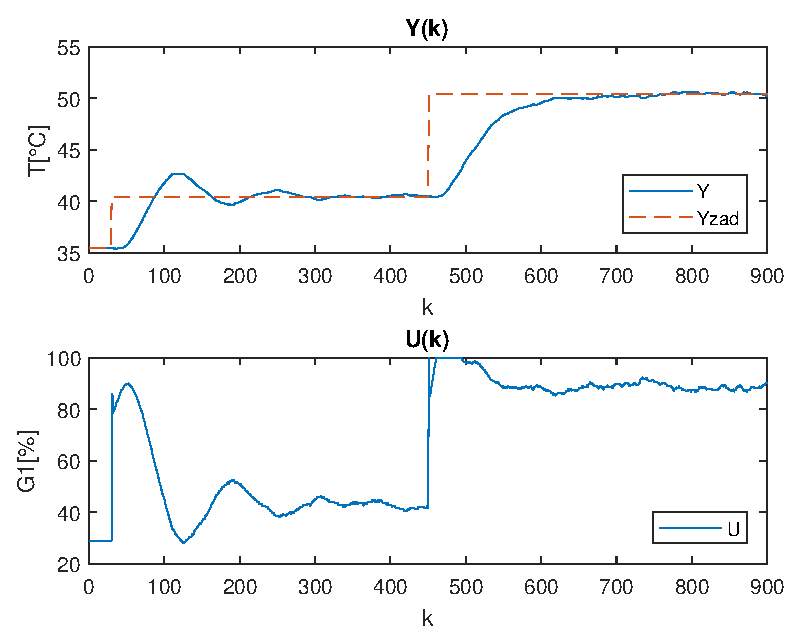
\includegraphics[scale=1]{Rys/NaiwnyPID.eps}
	\caption{Symulacja dla pojedynczego regulatora PID o parametrach $K=9,65, T_{i}=60,  T_{d}=0,17 $}
	\label{naiwnyPID}
\end{figure}


Błąd (suma kwadratów odchyłek) wyniósł E= \num{6077}.

\FloatBarrier

\section{Regulator DMC}

Wyniki symulacji przedstawiono na wykresie \ref{naiwnyDMC}:

\begin{figure}[h!]
	\centering
	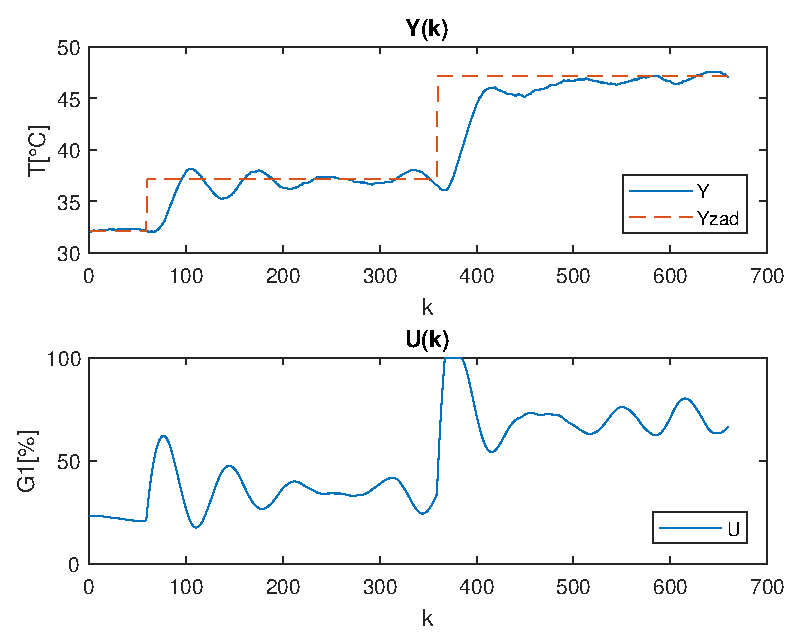
\includegraphics[scale=1]{Rys/NaiwnyDMC.eps}
	\caption{Symulacja dla pojedynczego regulatora DMC o parametrach $D=360, N=120, N_{u}=20, \lambda=1 $}
	\label{naiwnyDMC}
\end{figure}

Błąd (suma kwadratów odchyłek) wyniósł E= \num{3795} (wyniki można ze sobą porównywać mimo krótszego czasu trawnia symulacji, liczba skoków pozostała ta sama - tam są generowane głównie uchyby).

\section{Wnioski}

Pomimo że regulatory działają, temperatura zadana jest mniej więcej osiągana, jednak ich regulacja jest dosyć wolna, a wyjscie oscyluje. W celu poprawy regulacji dokonano rozmycia tych regulatorów.